%15 min preso!
\documentclass[xcolor=table,aspectratio=169]{beamer}
\usepackage{beamerthemesplit}
\usepackage{wrapfig}
\usetheme{SPbGU}
\usepackage{pdfpages}
\usepackage{amsmath}
\usepackage{cmap}
\usepackage[T2A]{fontenc}
\usepackage[utf8]{inputenc}
\usepackage[english]{babel}
\usepackage{indentfirst}
\usepackage{amsmath}
\usepackage{tikz}
\usepackage{multirow}
\usepackage[noend]{algpseudocode}
\usepackage{algorithm}
\usepackage{algorithmicx}
\usepackage{fancyvrb}
\usepackage{hyperref} 
\usetikzlibrary{calc}
\usetikzlibrary{shapes, backgrounds}
\usetikzlibrary{arrows,automata}
\usetikzlibrary{positioning}
\usetikzlibrary{fit}
\usetikzlibrary{shapes.callouts}
\usetikzlibrary{shapes.misc}
\usepackage{xparse}
\usepackage{fontawesome}

\usepackage{etoolbox,refcount}
\usepackage{multicol}

\usepackage{tabularx}
\newcolumntype{Y}{>{\raggedleft\arraybackslash}X}

\renewcommand{\thealgorithm}{}

\newtheorem{mytheorem}{Theorem}
\renewcommand{\thealgorithm}{}

\newcommand{\tikzmark}[1]{\tikz[overlay,remember picture] \node (#1) {};}
\def\Put(#1,#2)#3{\leavevmode\makebox(0,0){\put(#1,#2){#3}}}

\newcommand{\ltz}{$< 1$}

\tikzset{
    state/.style={
           rectangle,
           rounded corners,
           draw=black, very thick,
           minimum height=2em,
           inner sep=2pt,
           text centered,
           },
}

\tikzset{
    invisible/.style={opacity=0,text opacity=0},
    visible on/.style={alt=#1{}{invisible}},
    alt/.code args={<#1>#2#3}{%
      \alt<#1>{\pgfkeysalso{#2}}{\pgfkeysalso{#3}} % \pgfkeysalso doesn't change the path
    },
}

\tikzset{cross/.style={cross out, draw=black, minimum size=2*(#1-\pgflinewidth), inner sep=0pt, outer sep=0pt, ultra thick},
%default radius will be 1pt. 
cross/.default={1pt}}

\NewDocumentCommand{\mycallout}{r<> O{opacity=0.8,text opacity=1} m m m}{%
\tikz[remember picture, overlay]\node[align=center, fill=cyan!20, text width=#5cm,
#2,visible on=<#1>, rounded corners,
draw,rectangle callout,anchor=pointer,callout relative pointer={(290:0.5cm)}]
at (#3) {#4};
}

\NewDocumentCommand{\mycalloutR}{r<> O{opacity=0.8,text opacity=1} m m m}{%
\tikz[remember picture, overlay]\node[align=center, fill=cyan!20, text width=#5cm,
#2,visible on=<#1>, rounded corners,
draw,rectangle callout,anchor=pointer,callout relative pointer={(30:0.8cm)}]
at (#3) {#4};
}


%callout relative pointer={(230:0.5cm)}]

\newcounter{countitems}
\newcounter{nextitemizecount}
\newcommand{\setupcountitems}{%
  \stepcounter{nextitemizecount}%
  \setcounter{countitems}{0}%
  \preto\item{\stepcounter{countitems}}%
}
\makeatletter
\newcommand{\computecountitems}{%
  \edef\@currentlabel{\number\c@countitems}%
  \label{countitems@\number\numexpr\value{nextitemizecount}-1\relax}%
}
\newcommand{\nextitemizecount}{%
  \getrefnumber{countitems@\number\c@nextitemizecount}%
}
\newcommand{\previtemizecount}{%
  \getrefnumber{countitems@\number\numexpr\value{nextitemizecount}-1\relax}%
}
\makeatother    
\newenvironment{AutoMultiColItemize}{%
\ifnumcomp{\nextitemizecount}{>}{3}{\begin{multicols}{2}}{}%
\setupcountitems\begin{itemize}}%
{\end{itemize}%
\unskip\computecountitems\ifnumcomp{\previtemizecount}{>}{3}{\end{multicols}}{}}


\beamertemplatenavigationsymbolsempty

\title[ArkTS Parser]{Parsing Tools Research Proposal: ArkTS Parser}
\institute[SPbSU]{
Saint Petersburg State University
}

% То, что в квадратных скобках, отображается в левом нижнем углу.
\author[Semyon Grigorev]{Semyon Grigorev}

\date{2024}



\begin{document}
{
\begin{frame}[fragile]
  \begin{table}
  \centering  
  \begin{tabularx}{\linewidth}{XcX}
    
\includegraphics[height=0.9cm]{pictures/hu_logo.jpeg} \hfill
    & 
    & \hfill 
\includegraphics[height=1.6cm]{pictures/SPbGU_Logo.png}
  \end{tabularx}
  \end{table}
  \titlepage
\end{frame}
}

\begin{frame}[fragile]
  \frametitle{Why not existing tools?}  
  \begin{itemize}
    \item ANTLR
    \begin{itemize}
      \item[\faFrownO] Not incremental: it is unlikely possible to support accurate incremental parsing without totally rework
      \item[\faFrownO] No advanced error recovery 
    \end{itemize}
    \item TreeSitter
    \begin{itemize}
      \item[\faFrownO] Problems with error recovery
      \item[\faFrownO] Returns new ATS on input update: all your caches became useless
    \end{itemize}
    \item Babel + ANTLR = Current solution
    \begin{itemize}
      \item[\faFrownO] Poor performance
      \item[\faFrownO] Hard to extend grammar
      \item[\faFrownO] Not incremental
      \item[\faFrownO] No advanced error recovery 
    \end{itemize}
  \end{itemize} 
\end{frame}



\begin{frame}[fragile]
  \frametitle{Prpoposed solution}
  
  ArkTS parser on our own parsing infrastructure

  \vspace{1cm}
  
  Challenges:
  \begin{itemize}
    \item Nontrivial grammar (ambiguities, etc.)    
    \item Performance
    \item Error recovery    
    \item Incremental parsing
  \end{itemize} 
\end{frame}


\begin{frame}[fragile]
  \frametitle{Current State\footnote{\href{https://github.com/FormalLanguageConstrainedPathQuerying/UCFS/tree/cf_solver}{https://github.com/FormalLanguageConstrainedPathQuerying/UCFS/tree/cf\_solver}}}  
  \begin{minipage}{.45\textwidth}
  \begin{itemize}
    \item[\faCheck] Basic parser development tool
    \begin{itemize}
      \item[\faCheck] Grammar description DSL
      \item[\faCheck] Preliminary performance evaluation 
    \end{itemize}
    \item[\faCheck] Error recovery mechanism
    \begin{itemize}
      \item[\faGears] Preliminary performance evaluation 
    \end{itemize}
    \item[\faGears] User-friendly AST generation
  \end{itemize}
\end{minipage}
\begin{minipage}{.45\textwidth}
  \begin{itemize}
    \item[\faHourglassHalf] ArkTS parser development
    \begin{itemize}
      \item \href{https://github.com/antlr/grammars-v4/tree/master/javascript}{ANTLR grammar of TypeScript}
    \end{itemize}
    \item[\faHourglassHalf] Documentation
    \item[\faHourglassHalf] Performance tuning    
    \item[\faHourglassHalf] Advanced incremental parsing
  \end{itemize}
\end{minipage}
\end{frame}

\begin{frame}[fragile]
  \frametitle{Preliminary Evaluation Result}  
  \begin{itemize}
    \item Java grammar
    \item 3 real-world projects
    \begin{itemize}
      \item junit4: 425 files, avg. size 3KB (40KB max)
      \item guava:  1 416 files, avg size 8KB (198KB max)
      \item elasticSearch: 14 685 files, avg size 6KB (242KB max)
    \end{itemize}
  \end{itemize}
  \begin{center}
    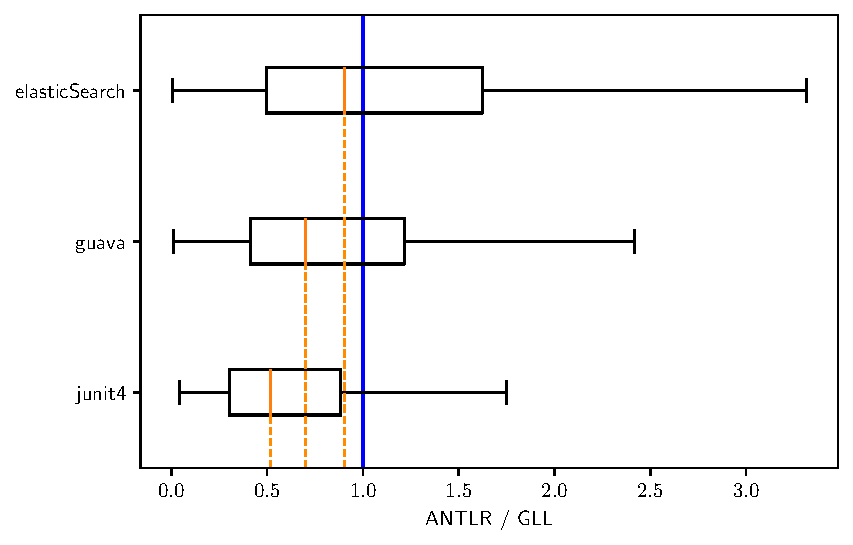
\includegraphics[width=0.5\textwidth]{pictures/gll_results.pdf}
  \end{center}
  
\end{frame}

\begin{frame}[fragile]
  \frametitle{Research Tasks}  
  \begin{itemize}
    \item Implement JavaScript subset parser 
    \begin{itemize}
      \item Evaluate performance of implemented parser
    \end{itemize}    
    \item Implement ArkTS subset parser 
    \begin{itemize}
      \item Evaluate performance of implemented parser
    \end{itemize}
    \item Performance tuning
    \item Grammars tuning
    \item Error recovery evaluation and tuning
    \item Incremental parsing implementation
  \end{itemize}  
  
\end{frame}



\end{document}
